% !TeX spellcheck = en_US
\color{fontcolor}
\begin{frame}
	Recommended reading:	
	\begin{itemize}
		\item Lecture 11 in \cite{TreBau}
		\item Section \texttt{II}.2 in \cite{StrangData}
		\item This handout by Homer F. Walker:\\ \href{https://users.wpi.edu/~walker/MA3257/HANDOUTS/least-squares_handout.pdf}{https://users.wpi.edu/$\sim$walker/MA3257/HANDOUTS/least-squares\_handout.pdf}
	\end{itemize}
	~\\~\\
	\bibliographystyle{plain}
	\bibliography{literature.bib}
\end{frame}

\begin{frame}
\Section{Least Squares Problems}
~\\
\Subsection{Overview}
~\\
\Hide{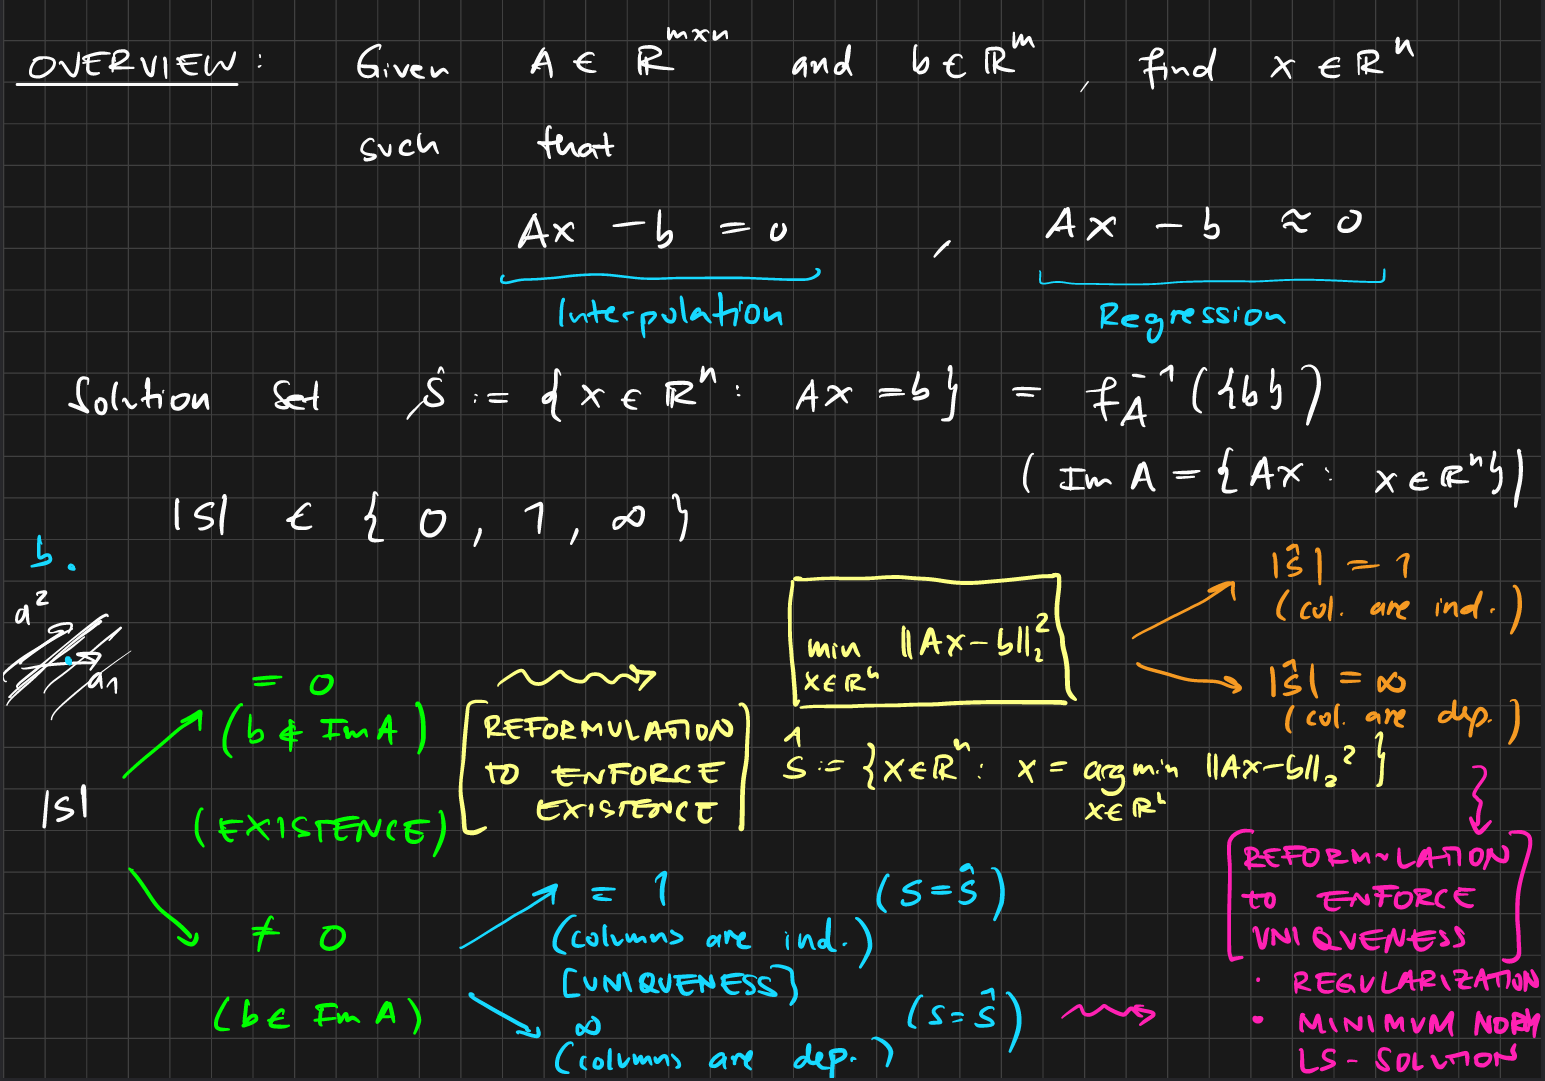
\includegraphics[width=0.8\textwidth]{overview-linsys.png}}
\end{frame}

\begin{frame}
	~\\
\textbf{Situation:} We allow for $b\notin \im(A)$\\ $\Rightarrow$ The system $Ax=b$ is not solvable, i.e., there is \textbf{no} $x^* \in \Rn$ so that $Ax^* = b$\\~\\
%
~\\
\textbf{Example:} Curve fitting\\
The situation above typically occurs when trying to explain a set of data by just a few parameters leading to over-determined systems: more equations than unknowns ($m  \gg n$).\\~\\
\begin{columns}[t]
	\begin{column}[t]{0.45\textwidth}
		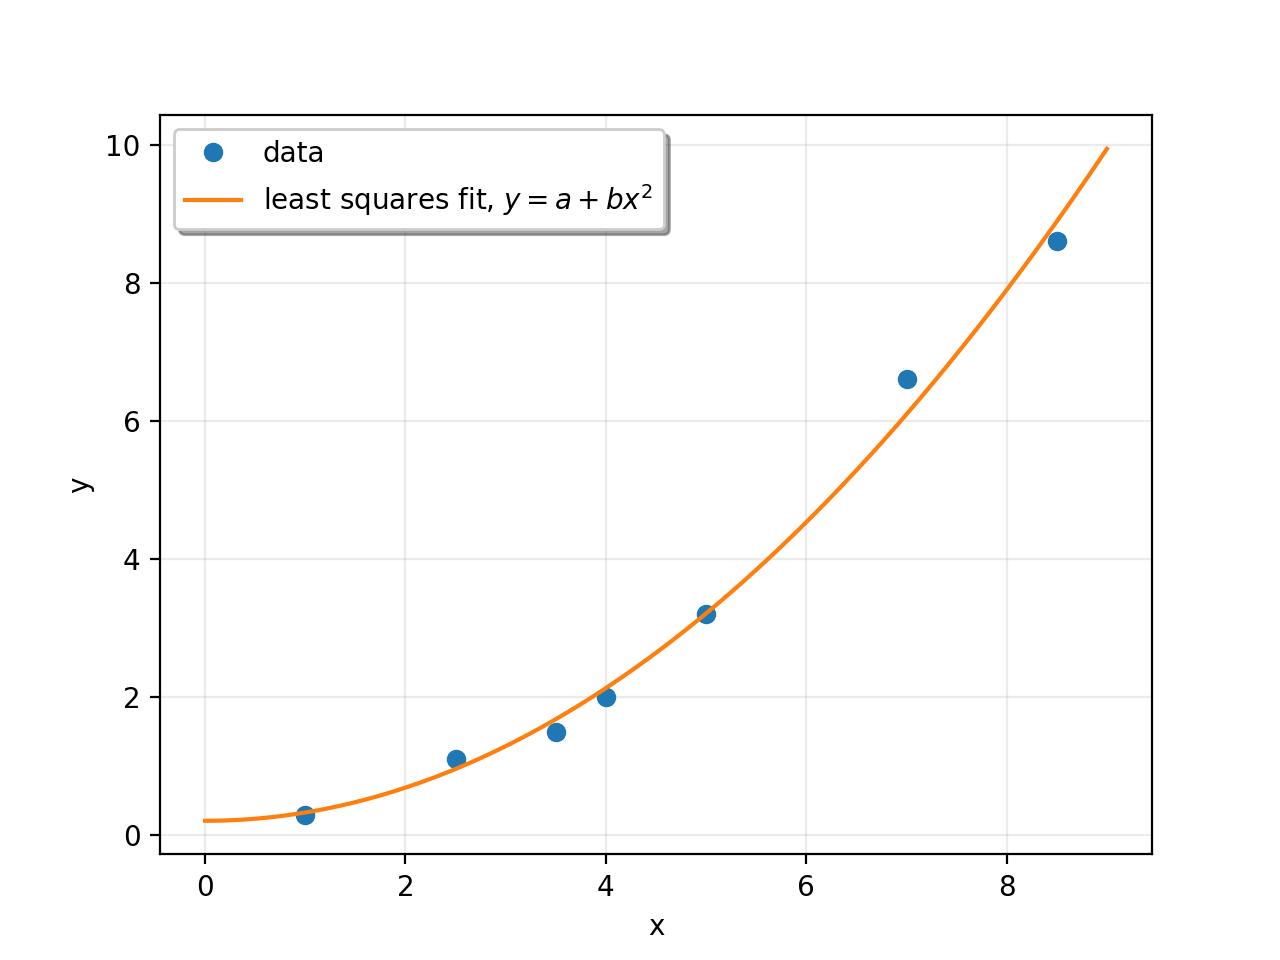
\includegraphics[width=0.99\textwidth]{4_least_squares.png}
	\end{column}
	\begin{column}[t]{0.45\textwidth}
	 \vspace{-4.6cm}~\\
	Corresponding system:
	$$
\begin{pmatrix}
		1&z_1^2\\
		\vdots & \vdots \\
		1&z_n^2
\end{pmatrix}	
\begin{pmatrix} 
a\\ b
\end{pmatrix}
 =
\begin{pmatrix}
	y_1\\ \vdots \\ y_n
\end{pmatrix}
$$
	\end{column}
\end{columns}
~\\



\end{frame}


\begin{frame}
~\\
%
\textbf{Approach:} Minimize the error (/residual/defect) $\|Ax-b\|$\\~\\
We obtain existence by reformulating the problem:

\begin{definition}[Least Squares Solution]
	Let $A \in \Rmn$ and $b \in \Rn$. Then $\widehat{x}\in \Rn$ is called a \textit{\textbf{least squares solution of $Ax=b$}}, if $\widehat{x}$ is a minimizer of the problem $$\min_{x\in\Rn} \|Ax - b\|_2^2,$$
	i.e., $\|A\widehat{x} - b\|_2^2 \leq \|Ax - b\|_2^2$ for all $x \in\Rn$.
\end{definition}
\Hide{
	~\\
	\textbf{Remark}
	\small
\begin{itemize}
	\item We recall that $\|x\|_2:=\sqrt{\sum_{i=1}^nx_i^2}$ which explains the naming: $$\|Ax-b\|_2^2=\sum_{i=1}^m\underbrace{(\dots)^2}_{\text{''\underline{squares}''}}\rightarrow\underbrace{\text{min}}_{\text{''\underline{least} squares''}}.$$
\item The norm is always nonnegative, i.e., $\|x\|_2\geq 0$, so that the minimal possible value of the objective function is zero (which would imply $Ax = b$ due to the definiteness of the norm). \\
\item Also, since squaring $x\mapsto x^2$ is a monotonically increasing function on nonnegative numbers we can minimize the squared residual without changing the set of minimizers, i.e., 
 $$\widehat{S}:=\{x\in\mathbb{R}^n:~x:=\arg\min_{x\in\mathbb{R}^n} \|Ax-b\|_{2}^{{\color{cyan}2}}\}= \{x\in\mathbb{R}^n:~x:=\arg\min_{x\in\mathbb{R}^n} \|Ax-b\|_2\}.$$
As a result we get rid of the square root which is advantageous in terms of derivatives (see optimality conditions later). Note that the optimal value of the objective function may differ, but this is not important here.
\end{itemize}
}
\end{frame}

\begin{frame}
\Subsection{The Normal Equation}
The minimization problem is equivalent to a linear system:
\begin{theo}[Normal Equation]
Let $A \in \Rmn$ and $b \in \Rm$. Then $\widehat{x}\in \Rn$ is a least squares solution of $Ax=b$ if and only if $\widehat{x}$ solves the \textit{\textbf{normal equation}} $$A^TAx = A^Tb. $$
\end{theo}
\textbf{Proof sketch:}
~\\~\\

\textit{(1) Optimization perspective:}\\~\\
\Hide{Let us define the objective function
$$f\colon \Rn \to \R, ~~f(x) := \|Ax - b\|_2^2.$$ 
Then one can show that $f$ is convex, i.e.,
$$f(\lambda x_1 + (1-\lambda)x_2)\leq \lambda f( x_1) + (1-\lambda)f(x_2)~~~\forall ~\lambda\in[0,1] .$$ In fact, this is an immediate consequence of the triangle inequality and the absolute homogeneity of the norm as well as the monotonicity of the square.\\~\\
The convexity of the objective function then implies the existence of a minimizer as well as the necessary \textit{and} sufficient first--order optimality condition:
$$\text{$\widehat{x}$ minimizer $\iff$ $0=f'(\widehat{x})=2A^T(A\widehat{x}-b)$ ~~(normal equation)} .$$
}
\end{frame}

\begin{frame}
\textit{(2) Geometric Perspective:}\\
~\\
\Hide{
	~\\
	We recall that 
	$$\im(A) = \{Ax\colon x\in\R^n\} = \text{span}(a_1,\ldots, a_n)= \{x_1 a_1 + \ldots + x_na_n\colon x\in\Rn\} \subset \R^m.$$
	Therefore the least squares problem also reads as
	$$\min_{x\in\Rn} \|Ax - b\|_2^2 = \min_{{\color{cyan}z\in\im(A)}} \|{\color{cyan}z}- b\|_2^2 .$$
	~\\
	\textbf{Example:} Let $A \in \R^{3 \times 2}$ and $b \in \R^3$.\\~\\
	\begin{minipage}{0.4\textwidth}
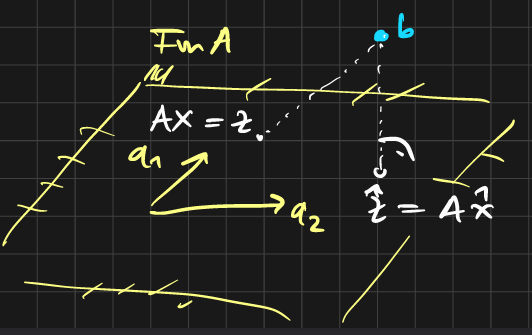
\includegraphics[width=\textwidth]{NormalEquationProof26-41} 
	\end{minipage}
\begin{minipage}{0.6\textwidth}
		\begin{itemize}
	\item The point $\widehat{z}\in\R^m$ ist the point in the plane $\im(A)$, which is as close as possible to $b$ in terms of the Euclidean norm $\|\cdot\|_2$.
	\begin{center}
		$\rightarrow$ The vector $(\widehat{z} - b)$ is orthogonal to this plane!
	\end{center}
\item By definition of the image $\im(A)$, each $z$ in this plane can be written as $z=Ax$ for some $x\in\R^n$.
\item The parameter vector $\widehat{x}$ with $\widehat{z}=A\widehat{x}$ is the desired least squares solution.
    \end{itemize}
\end{minipage}
	
	  
	}
\end{frame}

\begin{frame}
	One can show that the orthogonal projection yields shortest distance:
	\begin{lemma}[Orthogonal Projection]\label{lem:orthongonal-projection}
		Let $V \subset \R^m$ be a linear subspace and $b \in \Rm$. Then 
		$$\widehat{z}= \arg\min_{z\in V} \|z-b\|_2^2 ~~~\Leftrightarrow~~~ \widehat{z}-b \in V^\bot := \{w\in \Rn\colon w^\top z = 0~~ \forall z\in V\},~~\widehat{z}\in V . $$
	\end{lemma}
	\Hide{
		\begin{proof}
			The following equation is crucial for the proof (compare Pythagorean identity): Let $\widehat{z}\in V$ be fixed, then for all $z \in V$ we have
			\begin{equation}\label{eq:pythagorean_binomial}
			\begin{aligned}
			\|z-b\|_2^2 &= \|b-\widehat{z}+\widehat{z}-z\|_2^2\\
			&=\|b-\widehat{z}\|_2^2 + \|\widehat{z}-z\|_2^2 + 2(b-\widehat{z})^\top(z-\widehat{z})
			\end{aligned}	
			\end{equation}
			 ~\\~\\
			Exemplary, we only proof direction ``$\Leftarrow$'' here.\\
			Now let $\widehat{z}-b \in V^\bot$, so that $\forall z \in V$,
			\begin{align*}
			  (\widehat{z}-b)^\top(z-\widehat{z}) = 0.
			\end{align*}
			Inserting this into equation \eqref{eq:pythagorean_binomial} and exploiting the positivity of the norm we thus obtain
			\begin{equation*}
			\begin{aligned}
			\|z-b\|_2^2
			&=\|b-\widehat{z}\|_2^2 + \|\widehat{z}-z\|_2^2 + 2(b-\widehat{z})^\top(z-\widehat{z})\\
			&=\|b-\widehat{z}\|_2^2 + \|\widehat{z}-z\|_2^2\\
			&\geq \|b-\widehat{z}\|_2^2,
			\end{aligned}	
			\end{equation*}
			for all $z \in V$.\\~\\
			The reverse direction also relies on \eqref{eq:pythagorean_binomial}. See, e.g., the third proof  \href{https://en.wikipedia.org/wiki/Hilbert_projection_theorem\#Detailed_elementary_proof}{in this Wikipedia section}.
		\end{proof}
}
\end{frame}

\begin{frame}[c]
	Now let us apply this lemma to our setting $V = \im(A)$ and exploit the orthogonality of the fundamental subspaces ($\im(A)^\bot = \ker(A^\top)$). We obtain\\
	\Hide{	
		\begin{align*}
		\widehat{z}= \arg\min_{z\in \im(A)} \|z-b\|_2^2 & \iff ~~~ \widehat{z}-b \in \im(A)^\bot = \ker(A^\top),~~	\widehat{z}\in\im(A)~~~~~\text{\color{cyan}(Lemma \ref{lem:orthongonal-projection})}\\
		& \iff  ~~~A^\top(\widehat{z}-b) = 0,~~	\widehat{z}\in\im(A)~~~~~{\color{cyan}(\text{definition of $\ker(A^\top)$})} \\
		& \iff ~~~A^\top(A\widehat{x}-b) = 0 ~~~\text{for some}~\widehat{x}\in\Rn~~~~~{\color{cyan}(\text{definition of}~\widehat{z}\in\im(A))}
		\end{align*}
		~\\
		\begin{itemize}
			\item 		The normal equation then reads as:\\
			\begin{center}
				The least squares solution $\widehat{x}$ is so that \\
				the residual vector $A\widehat{x}-b$ is orthogonal to all columns of $A$.
			\end{center}
		~\\
			\item	We also find an equivalent characterization for the solution set, namely,\\
			$$\widehat{S} = \{x \in \Rn\colon A^TAx = A^Tb \}.$$ 
		\end{itemize}
	}
	 
\end{frame}

\begin{frame}
\textbf{Analysis of the Normal Equation}
~\\~\\
\textbf{(1)} Properties of the system matrix $A^TA$ (\textit{Gramian matrix})\\~\\ 
\Hide{
\begin{itemize}
	\item $A^TA$ is of size $n \times n$ (for typically $n \ll m$)%\\~\\
	\item $A^TA$ is symmetric and positive semi-definite {($\Rightarrow$ nonnegative eigenvalues)}%~\\
	\item $\ker(A) = \ker(A^TA)$, which implies:
	\item[] ~~~~~$A$ independent columns $\iff$ $\ker(A) = \{0\}$	{\color{red}$\iff$} $\ker(A^TA) = \{0\}$ $\iff$ $A^TA$ is invertible.\\~\\
	With other words, the least squares solution is unique if and only if $A$ has independent columns (also compare to the geometric interpretation above).
	~\\

\end{itemize}
}
	~\\~\\
\textbf{(2)} For any $A,b$ there exists a least squares solution (existence enforced $\checkmark$)\\~\\

\Hide{
	Due to %the symmetry of $A^TA$, 
	$\ker(A) = \ker(A^TA)$ and $\im(A) = \ker(A^T)^\perp$, we have
	\begin{align*}
	\text{existence:~}\exists x \in \Rn\colon A^TAx = A^Tb &\iff A^Tb \in \im(A^TA) = \ker(A^TA)^\perp = \ker(A)^\perp\\
	&\iff 0 = (A^Tb)^Tv = b^T(Av) ~~\forall ~v \in \ker(A)
	\end{align*}
	The latter statement on the right-hand side is true for any matrix $A$ and any vector $b$.	 }
\end{frame}


\begin{frame}~\\
\textbf{(3)} Consistent reformulation: \\
~\\
If $b \in \im(A)$, i.e., if the original system $Ax=b$ is solvable, then
$$\{x\in \Rn \colon Ax = b  \} =: S   = \widehat{S} := \{x\in \Rn \colon A^TAx=A^Tb  \}.$$
~\\~\\
 

\Hide{
	Proof:
\begin{itemize}
	\item ``$ S   \subset\widehat{S}$'':\\
	Let $x\in S=\{x\in\mathbb{R}^n:~Ax=b\}$ (such an element $x$ exists because we assume $b\in\text{Im}(A)$), then
	$$Ax-b=0~~
	\stackrel{A^T\cdot|}{\Rightarrow}~~A^T(Ax-b)=0~~
	\Rightarrow~~x\in \widehat{S}=\{x\in\mathbb{R}^n:~A^TAx=A^Tb\}.
	$$
	~\\
	\item``$ \widehat{S} \subset S$'':\\
	Let $\widehat{x}\in\widehat{S}$, i.e., $\widehat{x}:=\underset{x\in\mathbb{R}^n}{\mathrm{argmin}}\|Ax-b\|_2^2$, then \text{because}~$b\in\text{Im}(A)$,
	$$\|A\widehat{x}-b\|_2^2=0.$$
	Thus $$A\widehat{x}-b=0~~\Rightarrow~~\widehat{x}\in S.
	$$
\end{itemize}
	
}
\end{frame}



\begin{frame}
\Subsection{Solving the Normal Equation}
%
~\\
\textbf{Assumptions:} 
\begin{itemize}
	\item $A$ has independent columns (existence and uniqueness $\checkmark$)
	\item $n$ is of moderate size (direct methods applicable $\checkmark$)
\end{itemize}
%
~\\
Thus there is a unique least squares solution given by (also revisit the section on projections)
$$\widehat{x} = (A^TA)^{-1}A^Tb.$$
%
\textbf{Example:} Polynomial regression
\begin{itemize}
	\item Here we typically have many measurements $(z_1, y_1), \ldots, (z_m, y_m) \in \R^2$ (i.e., $m$ large).\\
	\item Polynomial model is given by $f_c(z) := \sum_{j=0}^{n-1}c_j z^j$ (for $n$ rather small because we want to smoothen the data).
	\item The corresponding design matrix is then given by $A = (z_i^{j-1})_{ij}$ (revisit section on curve fitting).\\
\item One can show:\\ \textit{\color{satzrot}If all the $z_i$ are distinct, then the columns of $A$ are independent (see \textit{Vandermonde matrix})!}
\end{itemize}

\Hide{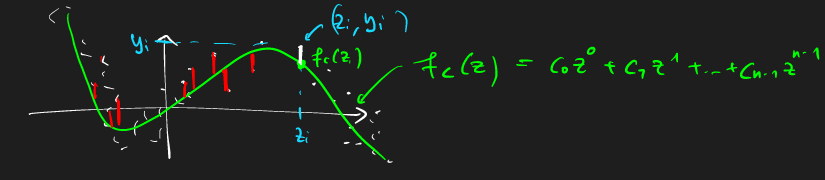
\includegraphics[width=\textwidth]{polynomial_regression.png}}
\end{frame}





\begin{frame}
	\textbf{Approaches:}\\~\\
	\textbf{(1)}\textbf{ Using Cholesky decomposition $A^\top A = LL^\top$}\\\vspace{0.2cm}
	%
	$\rightarrow$ Problem: $A^TA$ often \textit{ill-conditioned} and numerical elimination may fail due to rounding errors!\\ ~\\
%	(\textit{General note:} numerical difficulty in arithmetic operations is distinguishing exact zeros from small nonzeros)\\
	~\\
	\textit{Can we work without $A^TA$?} Yes!\\
	\textbf{(2)} \textbf{Using reduced $QR$ Decomposition $A = \widehat{Q}\widehat{R}$}\\
	\Hide{ \small
		Let us recall that $$	\forall A\in\mathbb{R}^{m\times n}~\exists~\widehat{Q}\in\mathbb{R}^{m\times n}~\text{orthonormal columns},~\widehat{R}\in\mathbb{R}^{n\times n}~\text{triangular}:~A=\widehat{Q}\widehat{R}.$$
		Now we insert $A=\widehat{Q}\widehat{R}$ into the normal equation to obtain
		$$
		A^TAx=A^Tb~~\stackrel{{\color{cyan}A=\widehat{Q}\widehat{R}}}{\Leftrightarrow}~~(\widehat{Q}\widehat{R})^T(\widehat{Q}\widehat{R})x=(\widehat{Q}\widehat{R})^Tb
		~~\Leftrightarrow~~\widehat{R}^T\widehat{Q}^T\widehat{Q}\widehat{R}x=\widehat{R}^T\widehat{Q}^Tb
		~~\Leftrightarrow~~\widehat{R}^T\widehat{R}x=\widehat{R}^T\widehat{Q}^Tb.
		$$
		If $A$ has independent columns, we know that $\widehat{R}$ is invertible and so is $\widehat{R}^\top$. Thus  we end up with the system 
		$$\widehat{R}x = \widehat{Q}^\top b $$
		which can be solved via \textit{backward substitution}.
		
		~\\
		\textit{Remarks:} \footnotesize
		\begin{itemize}
			\item Recall: Using the reduced $QR$ decomposition to solve $Ax=b$ results in the same system. Now we see that for the case $b \notin \im(A)$, we solve the normal equation.
			\item If the columns of $A$ are independent, then $\widehat{R}$ is invertible and without loss of generality one can require $r_{ii} > 0$, otherwise one multiplies the $i$-th column in $\widehat{Q}$ and row in $\widehat{R}$ by ``$-1$''. Thus, the factorization $\widehat{R}^\top \widehat{R}$ can be considered a Cholesky decomposition of $A^\top A$. However, the difference here is that we obtain it by the $QR$ decomposition of $A$ and not by applying the Cholesky algorithm to $A^\top A$. The former is roughly twice as expensive. One can show that this additional effort pays off in terms of improved stability against rounding errors.
		\end{itemize}
}
\end{frame}


\begin{frame}
	~\\
	\textbf{(3)} \textbf{Using the Pseudoinverse $A^+$} (see below)\\
	This is typically not done in practice since the computation of the singular value decomposition (which has to be iterative in higher dimensions since we need to solve eigenvalue problems) is more expensive than a direct method. However it offers interesting theoretical insights as we will see below.
	~\\~\\
	\textbf{(4)}\textbf{ Randomized algorithms:} \\
	If $A^TA$ is large ($n$ large), then in particular $A^TA$ cannot (and should not) be computed. \\
	In such cases one can use \textit{randomized} algorithms which only work with subsamples of the columns of $A$ (not addressed in this course; see for example \cite[II.4]{StrangData})\\ 
\end{frame}


%EXAMPLE
%
%\begin{ex}
%    Normal equations for straight line example:\\
%    \begin{equation*}
%        M = \begin{bmatrix}
%        1 & 1 \\
%        1 & 2 \\
%        1 & 3 \\
%        1 & 4 \\
%    \end{bmatrix},\; y = \begin{bmatrix}
%        10 \\
%        8 \\
%        9 \\
%        11 \\
%    \end{bmatrix}
%    \end{equation*}
%\bigskip
%
%normal equation: $\hspace{4cm} M^T Mp = M^T y$
%\begin{equation*}
%    M^T M = \begin{bmatrix}
%        1 & 1 & 1 & 1 \\
%        1 & 2 & 3 & 4 \\
%    \end{bmatrix} \begin{bmatrix}
%        1 & 1 \\
%        1 & 2 \\
%        1 & 3 \\
%        1 & 4 \\
%    \end{bmatrix} = \begin{bmatrix}
%        4 & 10 \\
%        10 & 30 \\
%    \end{bmatrix}
%\end{equation*}
%\begin{equation*}
%    M^T y = \begin{bmatrix}
%        1 & 1 & 1 & 1 \\
%        1 & 2 & 3 & 4 \\
%%    \end{bmatrix} \begin{bmatrix}
%        10 \\
%        8 \\
%        9 \\
%        11 \\
%    \end{bmatrix} = \begin{bmatrix}
%        38 \\
%        97 \\
%    \end{bmatrix}
%\end{equation*}
%\begin{equation*}
%    \left[ \begin{array}{cc|c}
%    4 & 10 & 38 \\
%    10 & 30 & 97 \\
%\end{array} \right] \longrightarrow \left[ \begin{array}{cc|c}
%    4 & 10 & 38 \\
%    0 & 5 & 2 \\
%\end{array} \right] \Longrightarrow p2 = 0.4, p1 = 8.5
%\end{equation*}
%\end{ex}
 
